\section{Approach}
\label{sec:approach}

Figure \ref{fig:architecture_overview} depicts the high-level processes of \splatter{} that execute when an integrated project is built. There are three major phases.

\textbf{Analysis.} Test run history is analysed and the probability of failure for each test is determined. Tests determined to be \flaky{} are prioritised in the next phase.

\textbf{Instrumentation.} \splatter{} extracts the packaged application, examines its bytecode and injects state-monitoring probes. Probe placement is informed by historical data, if available, and is performed with respect to an adaptive budget.

\textbf{Testing.} The test suite is run on the instrumented application; probes record events which are logged to files and stored in a database along with the test results after completion.

We first present our criteria for ranking \flaky{} tests (Section \ref{sec:sec:flakiness}). After defining our notion of budget (Section \ref{sec:sec:budget}) we then describe how budget is allocated on the test level, before zooming in to budget allocation on a bytecode level.

\begin{figure}[h]
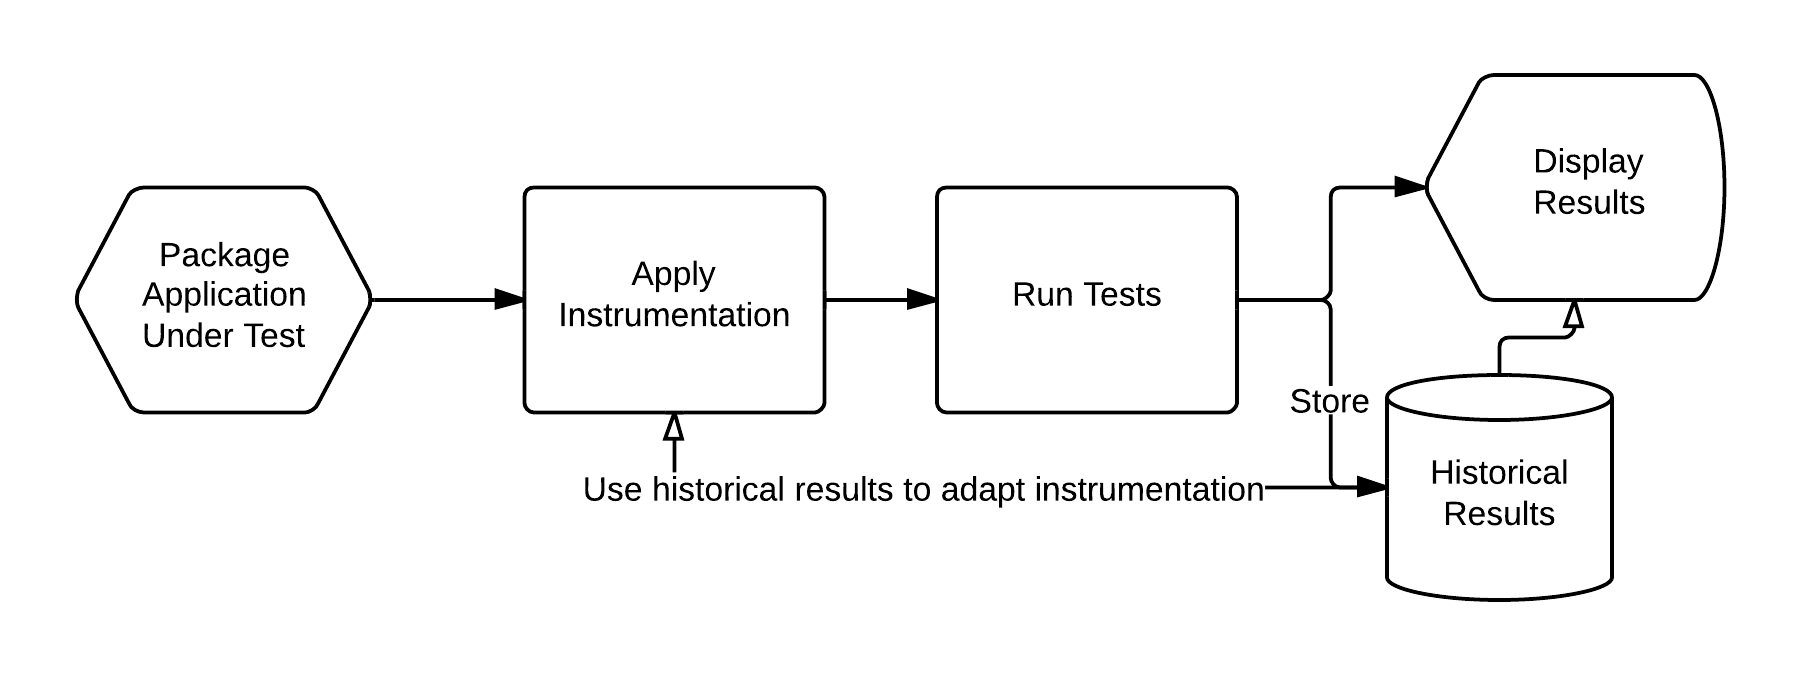
\includegraphics[width=\linewidth]{images/architecture_overview}
\caption{}
\label{fig:architecture_overview}
\end{figure}

\subsection{Flakiness}
\label{sec:sec:flakiness}

Each test is assigned a value in the range $[0..1]$, representing its flakiness. The higher the flakiness, the less likely the test is to fail on any given run. This value is used during test suite budget allocation.

\begin{figure}[here]\label{fig:app:flakiness}
\caption{}
	\begin{center}
		% See: http://www.texample.net/tikz/examples/line-plot-example/
		\begin{tikzpicture}[thick, framed, x=6.5cm, y=1.6cm]
			% Title
			\draw (0.5, 1) node[above] {$\textsc{\flaky{} Tests}$};

			% Axis
			\draw (0,0) -- coordinate (x axis mid) (1,0);
		    \draw (0,0) -- coordinate (y axis mid) (0,1);

		    % Axis Labels
		    \node (padding) [below] at (0.4, 0) {};
			\node[below of = padding] at (x axis mid) {Chance of Failure};

		    % Ticks
		    \foreach \x in {0, 0.4, 1}
		    	\draw (\x, 1pt) -- (\x, -3pt) node[anchor=north] {\x};
		    \foreach \y in {0, 1}
		    	\draw (1pt, \y) -- (-3pt, \y) node[anchor=east] {\y};

			% \flaky{} test range
		    \draw[<-] (0, 0.5) -- (0.4, 0.5); % Draw horizontal line
		    \draw (0.4, 0.42) -- (0.4, 0.58); % Draw right vertical tab

		    % Flakiness label
		    \node [above] at (0.2, 0.5) {$Flaky$};

		    % Alpha label
		    \node [right] at (0.4, 0.5) {$(\boldsymbol{\alpha})$};
		\end{tikzpicture}
	\end{center}
\end{figure}

Figure~\ref{fig:app:flakiness} shows the failure rates that qualify as \flaky{}. If a tests' chance of failure lies within the range $(0, \alpha]$, its flakiness value will be $(0, 1]$; otherwise, it will be $0$.

\todo{What value is $\alpha$, how do we calculate it? 0.4 is arbitrary!}
\todo{We ignore tests with failure rates greater than $\alpha$ since they could be reasonably reproduced by a developer?}

\algrenewcommand\algorithmicrequire{\textbf{Precondition:}}
\algrenewcommand\algorithmicensure{\textbf{Postcondition:}}

\begin{algorithm}[here]\label{alg:app:calculateFlakiness}
\caption{Calculating the flakiness of a test}
\begin{algorithmic}
	\Require{$chanceOfFailure$ and $threshold$ are decimal values within ranges $[0, 1]$ and $(0,1]$ respectively.}
    \Statex

	\Function{calculateFlakiness}{$chanceOfFailure$, $threshold$}

	\If{$chanceOfFailure \geq threshold$ OR $chanceOfFailure \eq 0$}
		\State \Return $0$
	\Else
		\State \Return $1 - (chanceOfFailure / threshold)$
	\EndIf

	\EndFunction
\end{algorithmic}
\end{algorithm}


\subsection{Test Suite Budget}
\label{sec:sec:budget}

There are two factors to take into account when determining our overall budget:

\begin{description}
	\item[Total time available] \hfill \\
 		Our upper bound for run time. This can be specified by the developer(s), or left as a sensible default.
	\item[Average run time of each test] \hfill \\
		Instrumentation comes with overhead. If we know the average run time of a suite without instrumentation and the estimated overhead of probes, we can apply instrumentation until we hit our upper bound. If we end up running over in practice, we simply reduce the budget and vice versa.
\end{description}

\todo{Test suite $f$ with \flaky{} tests $f!$.
Budget $B_{f} = B_{6} + B_{f!} + B_{nd}$}

\subsection{Allocating Test Suite Budget}

Test suite budget is distributed across all tests. We split our budget into two pools --- targeted and exploratory. We allocate targeted budget to tests with high flakiness, prioritising those with the highest flakiness and least historical data. Exploratory budget is randomly allocated to the remaining tests in the hopes that we get lucky and catch a previously stable test fail unexpectedly.

We start from a pesimistic; new tests are assumed to have a flakiness value of 1. As the test is run, the flakiness value is adjusted as usual until it represents a more accurate value. New tests will therefore be heavily instrumented, and gradually less so as they prove themselves to be reliable.

% The {algorithm} wrapper is pretty unattractive as far as I'm concerned.
% Need to look into alternative ways of formatting this.
\begin{algorithm}[h]
\caption{Instrumenting the test suite with respect to a budget}
\label{alg:splatter}
\begin{algorithmic}
	\Require{$tests$ is an set comprising all the tests in the test suite}
	\Require{$proportionTargeted$ is a decimal value in the range $[0, 1]$}
	\Statex

	\Function{splatter}{$tests$, $proportionTargeted$}

	\State $suiteBudget \gets$ calculateSuiteBudget($tests$)
	\Statex

	\State allocateBudget($tests$, $suiteBudget$, $proportionTargeted$)
	\Statex

	\ForAll {$test \in tests$}
		\State{instrument($test$)}
	\EndFor

	\EndFunction

	\Statex

	\Function{allocateBudget}{$tests$, $suiteBudget$, $proportionTargeted$}

	\State{$targetedBudget \gets suiteBudget * proportionTargeted$}
	\State{$exploratoryBudget \gets suiteBudget * (1 - proportionTargeted)$}
	\Statex

	\State{allocateTargetedBudget($tests$, $targetedBudget$)}
	\State{allocateExploratoryBudget($tests$, $exploratoryBudget$)}

	\EndFunction
\end{algorithmic}
\end{algorithm}

Algorithm \ref{alg:splatter} defines the two main steps: calculation and instrumentation. First a per-test budget is calculated based on our knowledge base; finally the instrumentation is performed. It is during the second step that the application is actually modified.


\subsubsection{Targeted Budget Allocation}

\begin{algorithm}[H]
\caption{Allocating targeted budget to tests}
\label{alg:allocateTargetedBudget}
\begin{algorithmic}
	\Function{AllocateTargetedBudget}{$tests$, $targetedBudget$}

	\State $totalFlakiness \gets 0$

	\ForAll{$test \in tests$}
		\State $totalFlakiness \gets totalFlakiness + test.flakiness$
	\EndFor
	\Statex

	\State $tests \gets \text{sortByFlakinessDescending(}tests$)

	\ForAll{$test \in tests$}
		\State $test.budget \gets$ calculateTestTargetedBudget($test$, $totalFlakiness$, $targetedBudget$)
	\EndFor

	\EndFunction
	\Statex
	\Function{calculateTestTargetedBudget}{$test$, $targetedBudget$}

	\State $maximumTargetedBudget \gets \todo{someNumberThatWeCalculate}$

	\State $budget \gets (test.flakiness / totalFlakiness) * targetedBudget$
	\Statex

	\Return minimum($testTargetedBudget$, $maximumTargetedBudget$)

	\EndFunction
\end{algorithmic}
\end{algorithm}

\subsubsection{Exploratory Budget Allocation}

\begin{algorithm}[h]
\caption{Allocating exploratory budget to tests}
\label{alg:allocateExploratoryBudget}
\begin{algorithmic}[1]
	\Function{AllocateExploratoryBudget}{ $tests$, $B_e$}

	\State shuffle($tests$)
	\State $iterator \gets tests.getIterator()$
	\While{$exploratoryBudget > 0$ AND $iterator.hasNext()$}
		\State $currentTest \gets tests.getNext()$
		\State \begin{varwidth}[t]{\linewidth}
		$exploratoryBudget \gets exploratoryBudget -$\par
		\hskip\algorithmicindent \text{calculateTestExploratoryBudget}(test, exploratoryBudget)
		\end{varwidth}
	\EndWhile

	\EndFunction
	\Statex
	\Function{CalculateTestExploratoryBudget}{test, exploratoryBudget}

	\State $maximumExploratoryBudget \gets \todo{someNumberThatWeCalculate}$

	\If{$test.budget > 0$}
		\Return $0$
	\EndIf

	\State $test.budget \gets$ minimum($exploratoryBudget$, $maximumExploratoryBudget$)

	\State \Return $test.budget$

	\EndFunction
\end{algorithmic}
\end{algorithm}


\subsection{Instrumentation}

\todo{Pseudocode should show instrumentation of an individual test based on previous instrumentation sites, budget, etc.}

\begin{algorithm}[H]
\caption{Instrument a test with respect its allocated budget}
\label{alg:instrument}
\begin{algorithmic}
	\State{\textbf{instrument} (test)}
	\State{$sites \gets test.instrumentationSites$}
	\While{$test.budget > 0$}
		\ForAll{$site \in sites$}
			\State{$cost \gets site.cost$}
			\If{$cost \le test.budget$}
				\State{$site.active \gets true$}
				\State{$test.budget \gets budget - cost$}
			\Else
				% Need to work out how to define new algorithmic-style macros (e.g. \BREAK)
				\State{\textbf{break}}
			\EndIf
		\EndFor
	\EndWhile
\end{algorithmic}
\end{algorithm}


\subsection{Monitoring Application State with Probes}

There are a number of types of points at which it is useful to gather information about application state. We extend the common approach of counters and predicates[] to include instrumentation designed for to gather much more contextual information.

We refer to a piece of code inserted at an instrumentation site to monitor application state as a probe. Complex probes record the state of live objects such as variables and method parameters, but carry a large performance overhead. Predicate probes are a lightweight alternative to monitor execution flow.

Probes are allocated based on the available budget, historical results and available instrumentation sites. For example, predicate probes could be used to hone in on program flows associated with failure during initial runs. Later, once areas of problematic code are identified, heavier-weight complex probes could then be inserted to gather more detailed information.

\todo{Dropped the ‘scalar value monitoring’ of previous approaches, since we can monitor a lot more with our budget when we are sure we’ve found an area of problematic code.}
\todo{Optimal placement of probes is NP-Hard?}

Complex probes serialize java objects to JSON with google-gson. Primitives are boxed to their object representations.

Predicate probes simply maintain a counter that is incremented each time the predicate is observed to be true.

\begin{center}
    \begin{tabular}{| l | p{6cm} | l |}
    \hline
        \textbf{Program Point} & \textbf{Description} & \textbf{Cost} \\
    \hline
        \multicolumn{3}{|c|}{\textit{Complex Probes}} \\
    \hline
        Function Entry &
        At the beginning of each function, we serialize all parameter objects (boxing primitives), along with all live variables. &
        \todo{Cost} \\
    \hline
        Function Return &
        At each function call with a return value, we serialize its object result. &
        \todo{Cost} \\
    \hline
        Conditional Branch &
        At each branch point, we record all variables in scope separately for each path. &
        \todo{Cost} \\
    \hline
        Variable Assignment &
        For an assignment $V = E$, where $E$ is an expression, we record both the current value of $V$ and the new value of $V$ after assignment. &
        \todo{Cost} \\
    \hline
        \multicolumn{3}{|c|}{\textit{Predicate Probes}} \\
    \hline
        Conditional Branch &
        At each path of the branch we maintain a counter that is incremented every time the path is taken. &
        \todo{Cost} \\
    \hline

    \end{tabular}
\end{center}


\subsection{Choosing Instrumentation Sites}

There are potentially millions of lines of code, where do we place our instrumentation?

Given an entry point, in our case, a test or setup method, we simply take the next set of code units in the control flow graph.

The main strategy is to place probes further and further down the control dependence graph until we are able to detect a failure-predicting predicate.

Once we have detected a failure-predicting predicate, we can assign the majority of our budget to drill down in related areas. Still, we reserve a portion to ‘scout’ in case we get lucky and find another failure predicting predicate elsewhere.
